\documentclass{jot}
% Use the documentclass option 'lineno' to view line numbers

% Enter the JOT metadata in the following 
\usepackage{multirow}

\jotdetails{
    volume=vv,      % volume
    number=nn,      % number or issue
    articleno=a1,   % article number, eg a1 for research articles, e for editorials
    year=2023,      % year
    license=ccby    % choose from ccby, ccbynd, ccbyncnd
}
\newcommand{\command}[1]{{\color{codepurple}\texttt{\textbackslash #1}}}
\newcommand{\param}[1]{{\color{blue}\texttt{#1}}}
% Select the article type
\articletype{regular} 
    % {editorial} editorial 
    % {regular} regular contribution
    % {manual} manual
    % {column} column

\title{Towards behavioral consistency in multi-modeling}

\author[$\ast$]{Tim Kräuter}
% Arbitrary co-author order. Everyone contributed significantly.
\author[$\ast\dagger$]{Harald König}
\author[$\ast$]{Adrian Rutle}
\author[$\ast$]{Yngve Lamo}
\author[$\ddagger$]{Patrick Stünkel}

\affil[$\ast$]{Western Norway University of Applied Sciences, Bergen, Norway}
\affil[$\dagger$]{University of Applied Sciences, FHDW, Hannover, Germany}
\affil[$\ddagger$]{Haukeland Universitetssykehus, Bergen, Norway}

\keywords{	
Global behavioral consistency,
Consistency verification,
Multi-modeling,
Heterogeneous models,
Rewriting Logic,
Graph transformation
}

\runningtitle{Towards behavioral consistency in multi-modeling} % For use in the internal pages 

\runningauthor{Kräuter \textit{et al.}}

\usepackage{amsthm} % for proofs
\usepackage{amsmath} % theorems, definitions, etc.
\newtheorem{definition}{Definition}
\newcommand{\definitionautorefname}{Definition}

\usepackage{glossaries}
\usepackage[nameinlink]{cleveref} % Reference footnotes.
\crefname{figure}{{figure}}{figures}
\Crefname{figure}{{Figure}}{Figures}
\crefformat{footnote}{#2\footnotemark[#1]#3}

\newacronym{ltl}{LTL}{Linear Temporal Logic}
\newacronym{mde}{MDE}{Model-Driven Engineering}
\newacronym{bpmn}{BPMN}{Business Process Modeling Notation}
\newacronym{uml}{UML}{Unified Modeling Language}
\newacronym{csp}{CSP}{Communicating Sequential Processes}
\newacronym{ccsl}{CCSL}{Clock Constraint Specification Language}
\newacronym{dsl}{DSL}{Domain-Specific Language}
\newacronym{srm}{SRM}{System Relationship Model}
\newacronym{gt}{GT}{Graph Transformation}
\newacronym{mt}{MT}{Model Transformation}
\newacronym{hot}{HOT}{Higher-Order model Transformation}
\newacronym{xdsl}{xDSL}{executable Domain-Specific Language}
\newacronym{mpm}{MPM}{Multi-Paradigm Modeling}
\newacronym{fsm}{FSM}{Finite State Machine}
\newacronym{dtds}{DTDS}{Discrete Time Discrete State System Specification}
\newacronym{devs}{DEVS}{Discrete Event System Specification}
\newacronym{fmi}{FMI}{Functional Mock-up Interface}
\newacronym{fmu}{FMU}{Functional Mock-up Unit}

% correct bad hyphenation here
\hyphenation{be-ha-vi-o-ral}

% Listing settings

\lstdefinelanguage{Interaction}[]{Java}{
    morekeywords={synchronize},
    comment=[l]{---},
}

\lstset{emph={  
    rl
    },emphstyle={\color{blue}\bfseries}
}


\begin{abstract}
Multiple heterogeneous interacting systems are needed to realize the requirements of complex domains.
Describing the interactions between these systems and checking their global behavioral consistency is a general, well-known challenge in software engineering.
To address this challenge, model-driven software engineering utilizes abstract representations of the constituting systems and their interactions, resulting in a \textit{multi-model} representing the overall system.
In such a multi-modeling setting, global consistency requirements must be satisfied by a set of heterogeneously typed models to guarantee a desired \textit{global behavior}.
In this paper, we propose a novel approach for behavioral consistency management of heterogeneous multi-models.
The approach introduces a workflow in which we
(i) define which behavioral models in the multi-model \textit{may interact},
(ii) specify consistency requirements as \textit{global behavioral properties},
(iii) align the individual models by specifying \textit{how they interact},
(iv) generate a formal specification of the \textit{global behavior}, and finally,
(v) \textit{check} the global behavioral properties, which should be satisfied by the multi-model.
Our approach is independent of the particular formalism used in the generated formal specification, and we currently support graph transformations (Groove) and rewriting logic (Maude).
\end{abstract}

\acknowledgment{We want to thank the anonymous reviewers for their valuable comments and helpful suggestions.}

\begin{document}    
\maketitle
\urlstyle{rm}

% TODO: Yngve remarks.
% TODO: consistency requirements in the abstract, behavioral consistency is defined by global behavioral properties. Make this clear and the language consistent.

\section{Introduction} \label{sec:introduction}
% Introduce multi-model
\gls*{mde} addresses the increasing complexity of software systems by employing models to describe the different aspects of the system.
In this way, \gls*{mde} promotes a clear separation of concerns and raises the abstraction level throughout the entire development process \cite{franceModeldrivenDevelopmentComplex2007}.
These models are then used to generate portions of the system leading to an increase in productivity and reduction of errors \cite{brambillaModeldrivenSoftwareEngineering2017}.
As multiple interacting systems are needed to realize the requirements of complex domains, a set of corresponding models would be needed to represent these systems and their interactions.
Such a collection of interrelated models is referred to as a \textit{multi-model} \cite{boronatWhatMultimodelingLanguage2009}, which is usually heterogeneous, meaning it consists of models conforming to different modeling languages.
% Consistency in multi-modeling
Models in a multi-model contradicting each other can lead to problems during development, system generation, and system execution.
Consequently, continuous multi-model consistency management during the development process is a significant issue for multi-models \cite{spanoudakisInconsistencyManagementSoftware2001, cicchettiMultiviewApproachesSoftware2019}.

% Consistency can be checked for a set of structural models
Recent research describes methods to check the structural consistency of a multi-model \cite{stunkelComprehensiveSystemsFormal2021, klareCommonalitiesPreservingConsistency2019}.
Structural models, like UML class diagrams, describe structural aspects of systems, i.e., domain concepts and relations between these concepts.
This is usually referred to as the denotational semantics of the software system, as it only describes the set of valid instances or states of the system.
Structural models in a multi-model often contain related information.
Thus, current approaches define so-called \textit{commonalities} to explicate these relationships and keep the information consistent.
Afterwards, these commonalities can be used to get a comprehensive view of the global system, for example, by \textit{merging} all models into a global view.
Structural consistency can then be verified using this global view.

% Challenge: Consistency for a set of behavioral models.
Nevertheless, approaches to multi-model consistency management must also include a means to maintain \textit{behavioral consistency} since behavioral models, like \gls*{bpmn} models, are associated with execution semantics describing dynamic aspects of the system \cite{objectmanagementgroupBusinessProcessModel2013}.
For example, multi-models consisting of different interacting behavioral models are used when modeling embedded and cyber-physical systems \cite{varalarsenBehavioralCoordinationOperator2015}.

% Existing solutions. But they are not sufficient!
Several approaches exist for checking the consistency of specific pairs of behavioral models.
For example, consistency checking for sequence diagrams and statecharts was implemented using Petri nets \cite{yaoConsistencyCheckingUML2006} and \gls*{csp} \cite{kusterExplicitBehavioralConsistency2003}.
Moreover, the co-simulation field tackles the simulation of interacting models by composing their individual simulations.
For example, by developing the \gls*{fmi} standard and implementing simulation tools such as Ptolemy \cite{ekerTamingHeterogeneityPtolemy2003}.
However, there is no approach to define and \textit{check consistency} of \textit{arbitrary many} behavioral models.

% Our approach summarized.
We propose a novel approach for consistency management of heterogeneous multi-models, which allows us to define and check \textit{global} behavioral properties.
Our approach facilitates specifying \textit{interactions} between multiple potentially heterogeneous behavioral models, which are used to generate a specification of the global behavior.
The approach is generally independent of the particular formalism used in the specification, and currently, we can generate specifications in two different formalisms.
The generation of the global behavior specification is \textit{fully automatic} and results in \gls*{gt} rules (or respectively, term rewriting rules) executable in Groove (Maude).
Afterward, we can use the built-in verification mechanisms in Groove (Maude) to check the previously defined global behavioral properties.

Our approach is based on two fundamental concepts: \textit{state} and \textit{state-changing elements}.
The state structure of each participating behavioral language must be explicitly defined such that we can infer how global states are structured.
Furthermore, state-changing elements must be identified in each participating behavioral language.
Thus, state-changing elements serve as a minimal \textit{behavioral interface} to uniformly define interactions for heterogeneous models.
Our approach applies to behavioral formalisms where these two concepts can be found which is the case for most formalisms with discrete state variables (see related work in \cref{sec:related_work}).

% Our approach related to structural consistency
The proposed approach partly resembles the state of the art approaches for structural consistency.
Interactions correspond to commonalities as both add necessary inter-model information.
Then, a global representation of the system's behavior/structure is constructed by composing the individual models using the interaction/commonality information.
Generating a global behavior specification is similar to merging structural models into a global view.
To achieve a global view for structural models, one introduces a base language in which individual models and the global view can be represented.
Likewise, generating our global behavior specification is based on the two fundamental concepts of \textit{state} and \textit{state-changing elements}.
In summary, we adapt the three steps for structural consistency management: Alignment, Verification, and Reconciliation as proposed in \cite{stunkelComprehensiveSystemsFormal2021} to a multi-model containing behavioral models.

% Paper outline
The remainder of this paper is structured as follows.
We introduce a simplified use case (\autoref{sec:usecase}) before explaining our behavioral consistency management approach in detail (\autoref{sec:behavioral_consistency_checking}).
Afterward, we show how we can use the \gls*{gt} toolset Groove to check behavioral consistency (\autoref{sec:specification_of_the_global_behavior}).
Furthermore, we discuss potential limitations of our approach in \autoref{sec:discussion}.
Finally, we examine related work in \autoref{sec:related_work} and conclude in \autoref{sec:conclusion_and_future_work}.


\section{Use Case} \label{sec:usecase}
This section motivates our approach with a simplified use case in which a traffic management system is developed to guide the traffic at a T-Junction with three traffic lights.
The traffic management system should control the traffic by switching between the two traffic phases highlighted in \cref{fig:junction-phases}.
In addition, it must fulfill the following two requirements.
First, it must guarantee safe traffic by correctly changing the three traffic lights, A, B, and C.
Second, it should prioritize arriving buses, i.e., switch the traffic lights quicker than usual to let an approaching bus pass (early green).
This so-called bus priority signal is a widely implemented technique to improve service and reduce delays in public transport.

\begin{figure}[h]
    \centering
    % warning is fine since it does not visually overflow.
    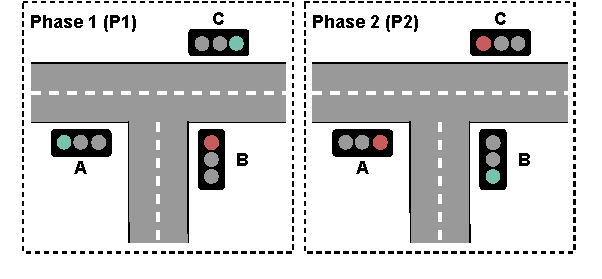
\includegraphics[width=0.5\textwidth]{figures/phases.pdf}
    \caption{Traffic phases of a T-Junction}
    \label{fig:junction-phases}
\end{figure}

To develop the behavior of the traffic management system, we follow an \gls*{mde} approach.
First, we model the behavior of a traffic light as a \gls*{uml} state machine.
Then we use \gls*{bpmn} to model the different traffic phases of the T-Junction, including the prioritization of approaching buses.

Using different behavioral modeling languages in the use case has two reasons.
First, two software development teams might work on the system in parallel but prefer different modeling languages.
Second, each team can choose the most appropriate modeling language for defining their part of the system.
In this use case, the behavior of a traffic light and a T-Junction differs significantly in complexity and requirements, resulting in the use of two different behavioral modeling languages, namely \gls*{uml} state machines, and \gls*{bpmn}.

The behavior of a traffic light is straightforward since it uses only three colors to guide the traffic.
\autoref{fig:trafficLight} shows a typical traffic light that switches from \textsf{red} to \textsf{red-amber}, \textsf{green}, \textsf{amber}, and back to \textsf{red}.
The start state of the traffic light in \cref{fig:trafficLight} is \textsf{red} but can be any of the four possible states.

\begin{figure}[h]
    \centering
    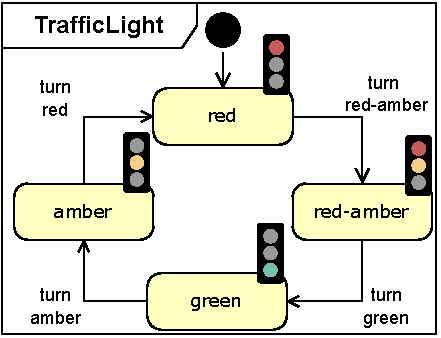
\includegraphics[width=0.35\textwidth]{figures/trafficLight.pdf}
    \caption{Traffic light state machine model}
    \label{fig:trafficLight}
\end{figure}

However, the T-Junction's behavior is more complex since it should coordinate the three traffic lights and communicate with approaching buses to implement bus priority.
Consequently, we are using \gls*{bpmn} to model this aspect of the system's behavior and utilize \gls*{bpmn} message and signal events to implement the communication with approaching buses.

We model two processes, one for the T-Junction and one for the Bus.
Each process is modeled in its \gls*{bpmn} \textit{pool}.
A pool is depicted as a horizontal lane with a name on the left.
Message flows (arrows with dashed lines) are only allowed between two different pools.

\autoref{fig:t_junction} shows how a possible controller for a T-Junction behaves in the traffic management system.
When a TJunction controller is started, we assume that the traffic lights are showing the colors according to phase 1 (see \cref{fig:junction-phases}).
Thus, the controller enters a subprocess called phase 1 (see top right in \cref{fig:communication}), which we describe together with the subprocess called phase 2 later.
However, when a fixed amount of time has passed, the subprocess is interrupted by the attached timer boundary event.
Then, the controller executes the next activity and switches to phase 2.
The controller will pass a throwing signal event before entering a subprocess for phase 2 and repeat the same steps.
This signal event represents a broadcast to all buses waiting for traffic light B to become green.
After switching back from phase 2 to phase 1 and signaling that traffic lights A and C are green, the controller can stop or execute the described steps again.
Typically, the controller does not stop, indicated by the default sequence flow going back to the beginning of the process.

% T-Junction BPMN model
\begin{figure*}[h]
    \centering
    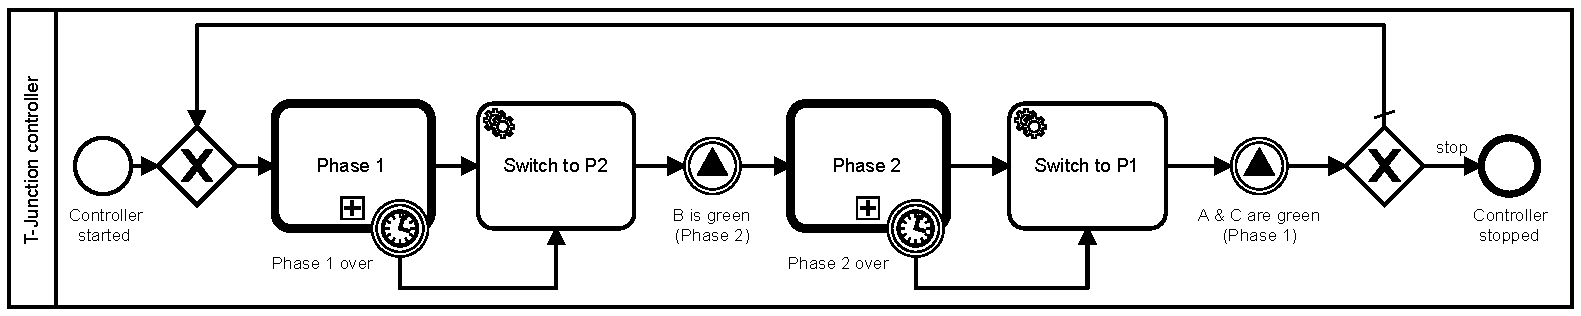
\includegraphics[width=1\textwidth]{figures/t-junction.pdf}
    \caption{Model for a TJunction controller}
    \label{fig:t_junction}
\end{figure*}

% Bus and Phase 1 BPMN model
\begin{figure*}[ht]
    \centering
    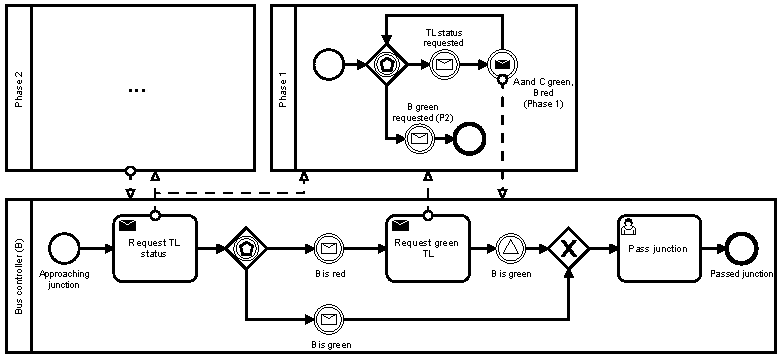
\includegraphics[width=1\textwidth]{figures/communication.pdf}
    \caption{Model for a bus with direction B and its communication with a T-Junction}
    \label{fig:communication}
\end{figure*}

\autoref{fig:communication} shows the communication of a bus with the subprocess phase 1.
The \gls*{bpmn} model and communication for phase 2 of the controller can be defined accordingly.

The phase 1 model uses an event-based gateway to respond to two different kinds of messages.
First, the traffic light status can be requested, which is answered by sending a message declaring that the traffic lights A and C are green while B is red.
Moreover, early green for traffic light B can be requested.
This request ends the subprocess, and the controller immediately switches to phase 2 (see \cref{fig:t_junction}), which results in the traffic light B turning green.

The bottom of \autoref{fig:communication} shows the controller for a bus parameterized with direction B.
It will first request the traffic light status to determine if traffic light B is green.
If it is green, the bus can pass the junction.
However, if it is red, the bus requests to change B to green and waits for a signal that the controller has changed the traffic light.
After receiving the signal, the bus passes the junction.
A \gls*{bpmn} model for a bus controller parameterized with the direction A or C looks nearly identical.
In addition, the bus controller communicates with the phase 2 subprocess, which we only hint at in \cref{fig:communication}.
The phase 2 subprocess has the same structure as the phase 1 subprocess but reports that A and C are red, while B is green.
Similarly, it terminates if green is requested for A or C.
The full model and all other models are available in \cite{krauterArtifactsBehavioralConsistency2023}.

Having developed behavioral models for the system, we want to check the previously stated \textit{safe traffic} requirement while buses are prioritized.
We can lower the overall development cost if we find bugs related to these requirements as early as possible during system development.
However, the traffic light model is currently not related to the T-Junction and bus models while the T-Junction is supposed to control the traffic lights, for example, when it switches between the two traffic phases.
In addition, the system has to manage multiple slightly different instances of the behavioral models.
For example, there are three traffic lights at one T-Junction starting in different states---i.e., showing different colors---and buses approaching the T-Junction from one of the three directions.
Consequently, we need a model of the system to allow us to define interactions between the models and configure instances of the behavioral models contained in the multi-model.

\begin{figure}[h]
    \centering
    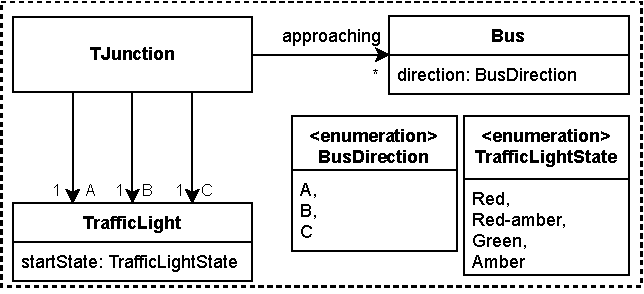
\includegraphics[width=0.45\textwidth]{figures/systemRelationShipModel.pdf}
    \caption{System relationship model of the traffic management system}
    \label{fig:systemRelationshipModel}
\end{figure}

The resulting model called the \textit{\gls*{srm}} is shown in \cref{fig:systemRelationshipModel} using a graph-based syntax.
It contains one node for each behavioral model and arrows to depict behavioral relationships, leading to possible interactions.
In addition, it contains enumerations to parameterize the behavioral models. 
A \textsf{TJunction} has three associated \textsf{TrafficLight}s, \textsf{A}, \textsf{B}, and \textsf{C}, and a set of currently approaching \textsf{Bus}es.
A \textsf{TrafficLight} has four possible \textsf{TrafficLightState}s and an attribute to define its \textsf{startState}.
A \textsf{Bus} has a \textsf{direction} that indicates which \textsf{TrafficLight} of the T-Junction it is approaching.

Finally, using the \gls*{srm}, we can define a test configuration of our traffic management system to check its requirements.
\autoref{fig:test_config} depicts the test system configuration as an instance of the \gls*{srm}.
First, it contains three instances of the traffic light behavioral model, representing the three traffic lights, \textsf{A}, \textsf{B}, and \textsf{C}.
Second, it contains an instance of the T-Junction behavioral model connected to the three traffic lights and two instances of the bus behavioral model.
Thus, the test system configuration describes a system that controls one T-Junction with three traffic lights and two buses approaching from directions A and B.

\begin{figure}[h]
    \centering
    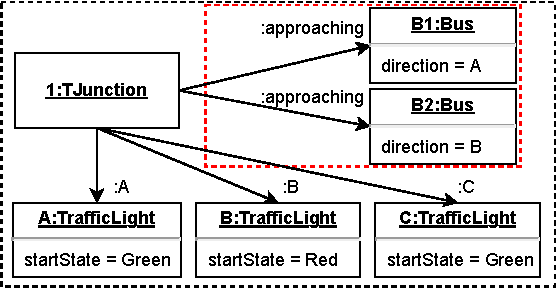
\includegraphics[width=0.45\textwidth]{figures/test_config.pdf}
    \caption{Test system configuration}
    \label{fig:test_config}
\end{figure}

First, we would like to check the safe traffic requirement.
Since we only want to check system conformance concerning the two traffic phases, we do not need to include the two buses depicted in the red dotted square in \cref{fig:test_config} in the analysis.
We cannot simply assert that the system is either in phase 1 or phase 2 since there are intermediate states during the transition between the two phases, which are allowed.
By consulting \cref{fig:trafficLight}, we can, for example, expect a state in which traffic lights A and C are amber, and traffic light B is red-amber before reaching phase 2.
However, we can define \textit{safe traffic} as the absence of \textit{unsafe traffic}, which is easier to define.

For the T-Junction, unsafe traffic occurs if traffic light A is green or amber and traffic light B is green or amber simultaneously.
In addition, the same state combinations are forbidden for traffic lights B and C.
Unsafe traffic occurs only in these situations since green and amber mean that cars are allowed to pass, while red (red-amber) means cars are not (not yet, respectively) allowed to pass.
We can formalize the consistency requirements as safety properties in \gls*{ltl}, i.e., states that should never be reached.
The resulting global properties \eqref{eq:property1} and \eqref{eq:property2} are the following, assuming the existence of atomic propositions for each traffic light state. 

\begin{align}
    \square\neg((A_{green} \lor A_{amber}) \land (B_{green} \lor B_{amber})) \label{eq:property1} \\
    \square\neg((C_{green} \lor C_{amber}) \land (B_{green} \lor B_{amber})) \label{eq:property2}
\end{align}

If we include buses \textsf{B1} and \textsf{B2} in the system, we would like to check that they cannot pass when their traffic light is red or red-amber.
Concretely, this means the \textsf{Pass Junction} activity should not execute while the corresponding traffic light is \textsf{red} or \textsf{red-amber}.
We formalize these requirements again by using \gls*{ltl} safety properties \eqref{eq:property3} and \eqref{eq:property4}, where the atomic proposition $B1_{passing}$ and $B2_{passing}$ represent that \textsf{Pass Junction} (see \cref{fig:communication}) has started but not finished yet.

\begin{align}
    \square\neg(B1_{passing} & \land (A_{red} \lor A_{red-amber})) \label{eq:property3} \\
    \square\neg(B2_{passing} & \land (B_{red} \lor B_{red-amber})) \label{eq:property4}
\end{align}

However, to check the global properties, we must execute the system with the behavior specified in the behavioral models according to the test configuration.
This is not straightforward since the multi-model of the use case consists of a \gls*{srm} relating two heterogeneously typed behavioral models.
In addition, the system configuration instantiates the traffic light and bus behavioral models multiple times with different parameters.
Furthermore, we face the problem that the models are not independent.
For example, the T-Junction controller must decide when the traffic lights A, B, and C switch states.
Thus, if we were to run the models independently in parallel, the properties would be violated.

A multi-model is behaviorally consistent if it satisfies all of its behavioral properties.
A behavioral property is given in temporal logic, for example, \gls*{ltl} in the use case, and is characterized as \textit{local} if it constrains only one model and as \textit{global} if it spans two or more models in a multi-model.
Furthermore, global properties depend on the system configuration, i.e., the instance of the \gls*{srm} used.
In the remainder of this paper, we will describe our approach to address behavioral consistency in multi-modeling and apply it to this use case.


\section{Behavioral consistency management} \label{sec:behavioral_consistency_checking}

\autoref{fig:approach} depicts our approach to behavioral consistency management as a \gls*{bpmn} diagram.

\begin{figure*}[h]
    \centering
    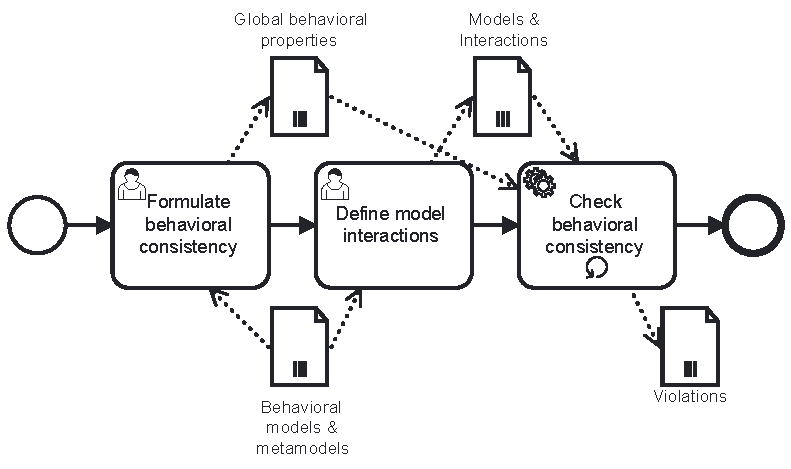
\includegraphics[width=0.7\textwidth]{figures/workflow.pdf}
    \caption{Behavioral consistency management workflow}
    \label{fig:approach}
\end{figure*}

Our approach consists of five steps.
\begin{enumerate}
    \item We define a \textit{\glsfirst*{srm}} describing which behavioral models may interact.
    \item We specify consistency requirements as global behavioral properties for the \gls*{srm}.
    \item We define \textit{interactions} between the behavioral models using the \gls*{srm}.
    \item We automatically generate a specification of the specified global behavior using the interactions and the \gls*{srm}.
    \item Given a system configuration, we check the global behavioral properties using the generated specification.
\end{enumerate}
The first three steps are marked as manual and must be completed to use our approach in a given use case.
However, the last two steps are automated and reusable without user intervention in any use case.
In the following sections, we will describe each step in detail, highlighting what a user must repeatedly do for each use case and what must only be done once for each participating behavioral language.
In addition, \cref{fig:allConcepts} at the end of the paper gives an overview of all the new concepts and how they are applied to the use case.


\subsection{Define the system relationship model}
As mentioned, a set of behavioral models might be used to describe the behavior of a software system.
Each model conforms to its metamodel, corresponding to the behavioral language used to specify the model.
The metamodel ensures that models specified in the corresponding languages are well-defined and machine-readable.
This is crucial when automating parts of the consistency checking.

The use case utilizes state machine and \gls*{bpmn} models, which conform, respectively, to the metamodels of state machines (see \cref{fig:fsm_metamodel}) and \gls*{bpmn} (see \cref{fig:bpmn_metamodel}).
The metamodel of state machines is defined by a \gls*{uml} class diagram.
In addition, the clouds depict the concrete syntax that we use to denote the models conforming to the metamodel.
The traffic light model in \cref{fig:trafficLight} uses this concrete syntax.

% state machine
\begin{figure}[h]
    \centering
    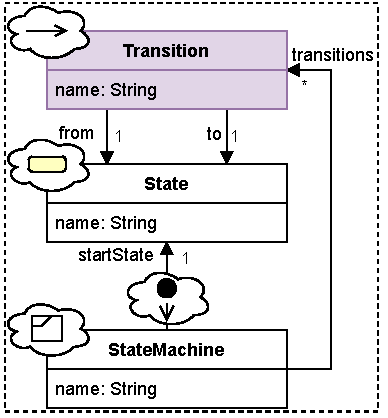
\includegraphics[width=0.275\textwidth]{figures/state_machine_metamodel.pdf}
    \caption{Finite state machine metamodel}
    \label{fig:fsm_metamodel}
\end{figure}

A \textsf{StateMachine} has a \textsf{startState} and \textsf{transitions}, whereas each \textsf{Transition} connects two \textsf{State}s.
The states of a state machine are not explicitly modeled but can be derived from the transitions of a state machine.
Furthermore, isolated states are not allowed.

The metamodel for \gls*{bpmn} (see \cref{fig:bpmn_metamodel}) is defined analogously to the one of state machines. 
A \gls*{bpmn} \textsf{Process} contains a set of \textsf{FlowNode}s connected by \textsf{SequenceFlow}s.
\textsf{FlowNode}s and \textsf{SequenceFlow}s are \textsf{FlowElement}s, inheriting an \textsf{id} and a \textsf{name}.
A \textsf{FlowNode} can be an \textsf{Activity}, \textsf{Gateway}, or \textsf{Event}.
All special activities, gateways, and events are defined in the \gls*{bpmn} specification \cite{objectmanagementgroupBusinessProcessModel2013}. % See BPMN class diagrams in figures 10.104/10.6/10.69.

% BPMN (a subset of the needed constructs)
\begin{figure}[h]
    \centering
    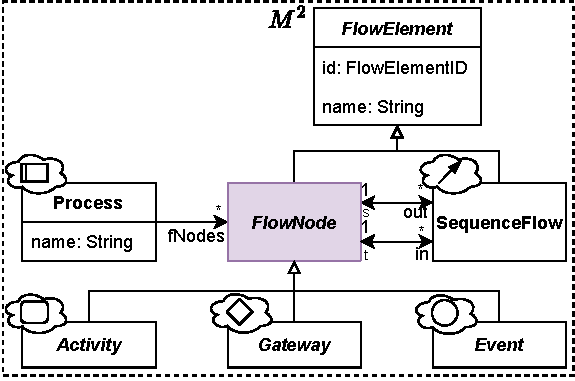
\includegraphics[width=0.475\textwidth]{figures/bpmn_metamodel.pdf}
    \caption{Simplified BPMN metamodel \cite{objectmanagementgroupBusinessProcessModel2013}}
    \label{fig:bpmn_metamodel}
\end{figure}

% System relationship metamodel
Behavioral models \textit{interact} to realize the global system behavior.
A \gls*{srm} describes which behavioral models exist in the system and whether they are behaviorally related, i.e., they may interact during execution.
In our approach, we define a system relationship metamodel to specify these relationships formally.
The constructed \gls*{srm} is use-case specific, while the metamodels for the participating languages must only be defined once.

We are using a graph-based syntax to define \gls*{srm}s (see \cref{fig:systemRelationshipModel}), where each node corresponds to a behavioral model (typed by a \textsf{BehavioralMetamodel}), while each arrow corresponds to a \textsf{BehavioralRelationship} (see concrete syntax depicted in clouds).
For example, the \gls*{srm} for the use case (see \cref{fig:systemRelationshipModel}) has three behavioral relationships from \textsf{TJunction} to \textsf{TrafficLight} since a TJunction controller interacts with three different traffic lights A, B, and C.
Furthermore, there is a behavioral relationship from \textsf{TJunction} to \textsf{Bus} because we want to check the safety properties \eqref{eq:property3} and \eqref{eq:property4}. 
To summarize, behavioral relationships define \textit{which} behavioral models \textit{may} interact, while the interactions in the next step of the workflow describe \textit{how} they interact.

In addition, we allow enumerations and attributes in \gls*{srm}s.
These may be used as parameters, e.g., to define the start state in a state machine (see \cref{fig:systemRelationshipModel}).
Different instances of the \gls*{srm} can be used to analyze the global behavior of \textit{different} system configurations by changing the parameters.

\subsection{Specify consistency requirements} \label{subsec:specify_consistency_requirements}
In this step, we specify behavioral consistency requirements as global behavioral properties.
These properties are defined using a temporal logic, for example, \gls*{ltl} as in the use case.
Theoretically, any temporal logic can be used together with our approach, however, in practice, the underlying system which runs the generated specifications must support it.
Furthermore, we agree with \cite{meyersProMoBoxFrameworkGenerating2014} that modelers are usually not familiar with temporal logic.
Thus, lifting property specification to the domain-specific level is a promising idea that fits our approach.
Nevertheless, for now, a modeler must define temporal logic properties.

Temporal logic properties are built upon a set of atomic propositions which are either true or false in a given state.
Each behavioral language (e.g., the BPMN) specification defines how these states are represented.
Furthermore, the transitions between these states depend on the semantics of the behavioral models.
In our approach, the first fundamental concept is to make \textit{state} structure explicit.
We will call the resulting models \textit{snapshot metamodels} and specify them using class diagrams.

For example, in the use case, we define snapshot metamodels for state machines and \gls*{bpmn}.
A state machine is in one state at a time, as shown in the snapshot metamodel on the left of \cref{fig:snapshot_metamodels}.
We are reusing the concrete syntax elements from the state machine metamodel (see \cref{fig:fsm_metamodel}) for the snapshot metamodel.
In addition, each snapshot metamodel has a root element in our approach, highlighted in light blue.
\begin{figure}[h]
    \centering
    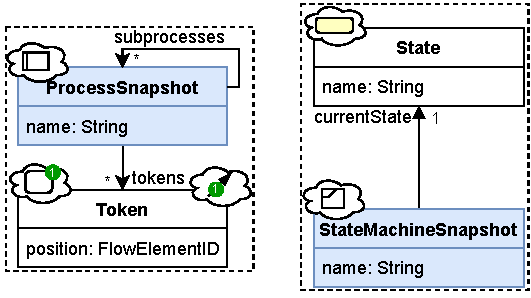
\includegraphics[width=0.4\textwidth]{figures/snapshot_metamodels.pdf}
    \caption{FSM and BPMN snapshot metamodels}
    \label{fig:snapshot_metamodels}
\end{figure}

The snapshot metamodel for \gls*{bpmn} is based on a \textsf{Token} distribution as described in the \gls*{bpmn} specifications \cite{objectmanagementgroupBusinessProcessModel2013} (see on the right of \cref{fig:snapshot_metamodels}).
The root element \textsf{ProcessSnapshot} has \textsf{tokens} and \textsf{subprocesses}.
A \textsf{Token} indicates where it is located in the \gls*{bpmn} model using its \textsf{position} attribute.
A valid \textsf{position} is the \textsf{id} of a \textsf{FlowElement} (see \cref{fig:bpmn_metamodel}).
Also, for the snapshot metamodel of \gls*{bpmn} we reuse the concrete syntax of the \gls*{bpmn} metamodel.
In addition, \textsf{Token}s are highlighted with green bubbles in the middle of sequence flows and the top right of an activity.

Each instance of a snapshot metamodel can represent an atomic proposition since a system can either be in the state specified by this instance or not.
Since instances of snapshot metamodels are essentially graphs, they can be matched to a given system state uniformly.
Thus, using the snapshot metamodels to create atomic propositions, we can specify local behavioral properties for any modeling language.
However, to specify global behavioral properties, we must combine the information of the \gls*{srm} with the snapshot metamodels.
Each behavioral model is typed by a behavioral metamodel, which has a snapshot metamodel describing its state structure.
Thus, we know how states of behavioral models are represented when they are instantiated.
For example, \cref{fig:atomic_propositions} shows how to specify the atomic propositions $A_{green}$ and $B1_{passing}$, used in the global properties in \autoref{sec:usecase}.
Snapshot links connect instances of behavioral models with root element instances of the corresponding snapshot metamodel. 

\begin{figure}[h]
    \centering
    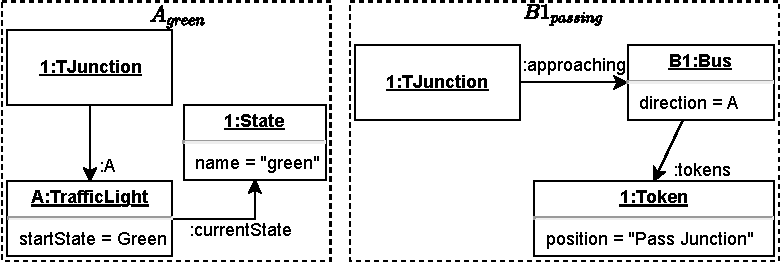
\includegraphics[width=0.475\textwidth]{figures/atomic_props.pdf}
    \caption{Atomic propositions $A_{green}$ and $B1_{passing}$}
    \label{fig:atomic_propositions}
\end{figure}

To make formulating atomic propositions less cumbersome, one can use the concrete syntax of the individual snapshot metamodels.
For example, \cref{fig:atomic_propositions_concrete} shows the same atomic propositions as \cref{fig:atomic_propositions} but uses the introduced concrete syntax.

\begin{figure}[h]
    \centering
    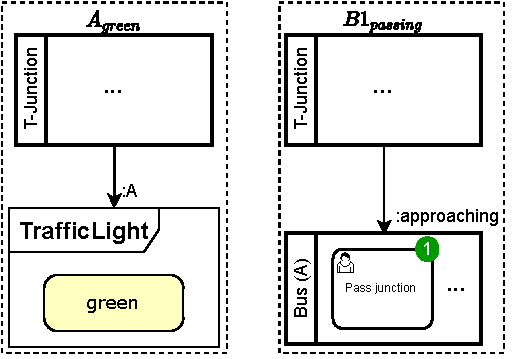
\includegraphics[width=0.375\textwidth]{figures/atomic_props_concrete.pdf}
    \caption{Concrete syntax for $A_{green}$ and $B1_{passing}$}
    \label{fig:atomic_propositions_concrete}
\end{figure}

With the defined atomic propositions as ingredients, one can use temporal logic to define global behavioral properties such as the properties \eqref{eq:property1}-\eqref{eq:property4} in \autoref{sec:usecase}.
It is worth noting that the defined atomic propositions are \textit{model-specific}, meaning they exactly fit the given multi-model.
Thus, property definition (including atomic propositions) is done for each use case, while snapshot metamodels for behavioral languages must only be defined once.

\subsection{Define model interactions}
We call behavioral inter-model relationships \textit{interactions} since they carry behavioral meaning while commonalities carry structural meaning \cite{stunkelComprehensiveSystemsFormal2021, klareCommonalitiesPreservingConsistency2019}.
To specify interactions between different behavioral models, we define an interaction language given by the system relationship metamodel in \cref{fig:srm_metamodel}.
In addition, we introduce the second fundamental concept of \textit{state-changing elements}.
Each \textsf{BehavioralMetamodel} specifies a set of \textsf{StateChangingElement}s.
For example, a state machine defines states and transitions, but only the transitions describe how the states in a state machine change.
Thus, the transitions are the state-changing elements of a state machine (highlighted in purple, see \cref{fig:fsm_metamodel}).
Similarly, the flow nodes are the state-changing elements of a \gls*{bpmn} process (highlighted in purple, see \cref{fig:bpmn_metamodel})\footnote{One exception is the event-based gateway, which is not part of the state-changing elements.}.
The interaction of behavioral models is only possible through instances of state-changing elements.
Thus, state-changing elements function as a minimal \textit{behavioral interface} to define interactions for heterogeneous behavioral languages uniformly.

Our approach is based on the requirement that state-changing elements can be identified in metamodels for any used behavioral formalism.
This requirement is not difficult to meet since behavioral modeling languages with a discrete state must have some \textit{observable} construct to describe state changes.
Inspecting other behavioral languages, such as Petri Nets or activity diagrams, shows that identifying state-changing elements (transitions and activity nodes, respectively) is unproblematic. 

\begin{figure}[h]
    \centering
    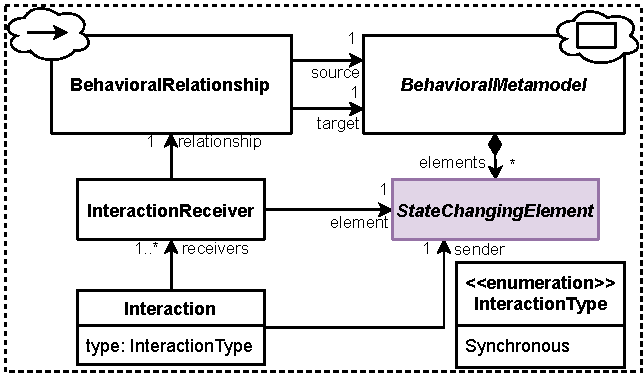
\includegraphics[width=0.45\textwidth]{figures/srm_metamodel.pdf}
    \caption{System relationship metamodel}
    \label{fig:srm_metamodel}
\end{figure}

An \textsf{Interaction} has a \textsf{sender}, a set of \textsf{receivers}, and a \textsf{type}.
Currently, there is only the \textsf{synchronous} \textsf{InteractionType}.
However, more interaction types, for example, asynchronous interactions or interactions with message passing, could be added in the future.
We model the role of sender and receiver in interactions to accommodate these interaction types in the future.
The two roles are not needed for synchronous interactions and are hidden from the user in the concrete syntax used later in \cref{lst:interactions}.
Furthermore, asynchronous interactions can be modeled using two synchronous interactions with an additional behavioral model, such as a queue.
Each \textsf{InteractionReceiver} references one \textsf{BehavioralRelationship} and one \textsf{StateChangingElement}.

Adding new interaction types only impacts steps 3.3 and 3.4 in our approach (see \cref{fig:approach}).
Concretely, a new interaction type has to be added to the enumeration in the system relationship metamodel and must be accounted for in the concrete syntax for interactions.
Then, the semantics of the new interaction type must be added to the generation of the global behavior specification in step 3.4. 

The \textsf{sender} and the elements of the \textsf{InteractionReceiver}s describe a state change for their behavioral models.
By connecting them with a synchronous interaction, we define simultaneous state changes in one atomic step. 
Consequently, an interaction defines a synchronization between behavioral models.
Generally, models behave in a distributed independent fashion until they reach a state-changing element that is part of an interaction.
To execute these state changes, the models must then interact, i.e., synchronize as described.
In addition, one can only define interactions for state-changing elements if a behavioral relationship connects their behavioral models (see constraint \eqref{eq:interactionConstraint}).
We use "." in constraints to navigate along associations.
For example, \textsf{i.receivers} means following all \textsf{receivers} links for an \textsf{Interaction} object, resulting in a set of \textsf{InteractionReceiver} objects.

\begin{equation} \label{eq:interactionConstraint}
    \begin{aligned}
    & \forall i \in Interaction: \forall r \in i.receivers : \\
    & \quad r.element \in r.relationship.target.elements \; \wedge \\
    & \quad i.sender \in r.relationship.source.elements
    \end{aligned}
\end{equation}

We allow the definition of as many interactions as desired.
Two interactions are not allowed to share state-changing elements (see constraint \eqref{eq:noOverlap}).
If such a situation occurs, it must be resolved by the modeler by deleting one of the interactions or merging the two interactions into one.

\begin{equation} \label{eq:noOverlap}
    \begin{aligned}
    & \forall i_1,i_2 \in Interaction : \\
    & \quad (i_1.receivers.element \cup i_1.sender) \; \cap \\
    & \quad (i_2.receivers.element \cup i_2.sender) = \emptyset
    \end{aligned}
\end{equation}

In the use case, the TJunction controller interacts with the three traffic lights, \textbf{A}, \textbf{B}, and \textbf{C}.
\autoref{lst:interactions} defines two interactions synchronizing TJunction controller and the traffic lights, using a textual \gls*{dsl}.
The \textbf{synchronize} keyword specifies the \textsf{InteractionType} to be \textsf{synchronous}.
Each interaction first defines the \textit{sender} state-changing element.
Then \textit{receivers} are defined by navigating along an arrow (\textsf{BehavioralRelationship}) to other \textsf{BehavioralModel}s in the \gls*{srm} and then specifying a \textsf{StateChangingElement}.
All navigation along \textsf{BehavioralRelationship}s starts from the \textsf{BehavioralModel} containing the \textit{sender}, so constraint \eqref{eq:interactionConstraint} is fulfilled.

\lstinputlisting[
label=lst:interactions,
language=Interaction,
caption=Interactions for the use case]{figures/interactions.txt}

We can explain the interactions as follows.
The first interaction defines that the task \textsf{Switch to P1} and three other state-changing elements synchronize.
Furthermore, line 2 specifies that one of the synchronization receivers is the element \textit{turn green} connected by the relationship \textit{A}.
Similarly, two other transitions of the traffic lights \textit{B} and \textit{C} are specified in the following two lines.
Thus, the interaction defines a synchronization of a task and three traffic light transitions. 
The second interaction defines a synchronization for the task \textsf{Switch to P2} and three traffic light transitions.

To summarize, we use the system relationship metamodel to define the relations between the behavioral models in a multi-model.
Thus, the inter-relations between behavioral models in a multi-model are given by interactions and their behavioral relationships.
Interactions are specific to each use case, but identifying state-changing elements must only be done once for each behavioral language.

\subsection{Generate a global behavior specification}
Using the \gls*{srm} and snapshot metamodels, we can represent the global states of the system.
However, we still need a formal specification of the global behavior to check the defined properties.
The specification of the global behavior used in our approach must fulfill the following three requirements:
\begin{enumerate}
    \item The specification must respect the semantics of each behavioral model.
    \item The specification must reflect the defined interactions between the behavioral models.
    \item The specification semantics must allow the checking of behavioral properties for a given system configuration.
\end{enumerate}
Thus, a specification in any formalism fulfilling these three requirements can be used in our approach.
Consequently, one can experiment with different formalisms, for example, \glspl*{gt}, rewriting logic, state machines, Petri nets, or process algebras, without changing the general framework.
One can then pick the most suitable formalism for the modeling scenario at hand regarding, for example, the performance of consistency checking.
In \cref{sec:specification_of_the_global_behavior}, we describe how we generate specifications for the \gls*{gt} toolset Groove.

To summarize, we generate a specification of the global system behavior.
This generation takes the models and interactions as input and is fully automated to allow frequent model changes.


\subsection{Check behavioral consistency}
% Model checking for a system configuration
In this step, for a given system configuration, we use the generated specification of the global behavior to check consistency.
A system configuration is an instance of the \gls*{srm} and is automatically translated into the formalism used in the specification.
We then check the defined properties using the specification and the system configuration.
This step is fully automated, such that it can be executed as many times as needed for different system configurations and properties while using the same specification.

Finally, a violation, including a counterexample, will be presented if a consistency requirement is not fulfilled.
We can only show counterexamples if the concrete tool, executing the generated specifications, provides them.
However, most modern tools, including Groove and Maude, will provide a counterexample.
Adopting the same concrete syntax to visualize the counterexample as for the atomic propositions should be ideal for helping user understanding. 
An unsuccessful consistency check leads to a consistency restoration process, which is crucial but out of the scope of this paper.
We describe consistency checking for the use case and its result at the end of the next section.


\section{Specification of the global behavior} \label{sec:specification_of_the_global_behavior}
In this section, we will describe our implementation to generate formal \gls*{gt} specifications for Groove \cite{rensinkGROOVESimulatorTool2004}.
Then, we use the generated specification to check behavioral consistency for the use case and discuss the results.
We have chosen to use the \gls*{gt} formalism to describe our approach because \glspl*{gt} provide a visual representation and allow for a clearer understanding.
Additionally, a description of the term-rewriting implementation in Maude is part of the artifacts of this paper \cite{krauterArtifactsBehavioralConsistency2023}.

Both implementations utilize a \textit{global} \gls*{hot} from the behavioral models and their interactions to \gls*{gt} rules (Groove) or term rewriting rules (Maude).
Since the results of the \gls*{mt} can be regarded as \gls*{mt}s themselves, we say the \gls*{mt} is \textit{higher-order} \cite{tisiUseHigherOrderModel2009}.
In the following, we describe the \gls*{hot} to generate \gls*{gt} specifications for Groove.
The \gls*{hot} works similarly when generating a term-rewriting specification for Maude.

The \gls*{hot} can be decomposed into two steps.
The first step to generate a specification of the global behavior is to create \gls*{gt} rules for each behavioral model contained in the multi-model.
Each set of rules must describe the behavior of the given behavioral model by manipulating instances of the snapshot metamodels.
For example, a rule for a transition in a state machine changes the current state of a state machine snapshot from the source to the target of the transition. 

Thus, we need \textit{local} \gls*{hot}s for each behavioral modeling language producing rules.
Each local \gls*{hot} only has to be implemented once by an \gls*{mde} tool developer.
The \gls*{hot}, metamodel and snapshot metamodel for a behavioral language can be shared together, for example, as a plugin, such that they can be reused in any future setting the language is needed.
In addition, each local \gls*{hot} must keep traces of the generated rules.
Concretely, it has to save which rules originated from which state-changing elements in the behavioral model.
Returning to the state machine example, we must know which transition results in which rule.
In general, multiple rules may be associated with one state-changing element of a behavioral model.
For example, a receive task in a \gls*{bpmn} process is represented by two rules since it starts and then waits for an incoming message before finishing.

The second step is to modify the generated rules to reflect the defined interactions.
Interactions define the synchronization of systems, which we encode by merging the individual rules into rules describing the global behavior.
The merging process to obtain the global rules is done in two steps:

\begin{enumerate}
    \item Rules generated from state-changing elements that are \textit{not} part of interactions remain unchanged and are added to the global rule set.
    \item For each interaction, we do the following:
     \begin{enumerate}
         \item Find the corresponding rule\footnote{If one state-changing element results in more than one rule, one can define a strategy to pick the appropriate rule.} $P_0$ for the sender of the interaction and find the rules $P_1, P_2, \ldots P_n$ for the receiver state-changing elements using the saved traces.
         \item Create a \textit{global rule} for the rules $P_0, P_1, \ldots, P_n$, which applies all of them at once, i.e., synchronizes the state changes of the behavioral models.
         \item For each receiver of the interaction, instantiate the corresponding behavioral relationship from the behavioral model in $P_0$ to the behavioral model in $P_i$, for 1 $\leq$ i $\leq$ n, and add it to the global rule.
         Thus, only behaviorally related models may interact, i.e., change their state simultaneously.
     \end{enumerate}
\end{enumerate}

\Cref{fig:global_rule} shows the global rule resulting from the merging process for \gls*{gt} rules.
The global rule contains four individual rules changing the state of three traffic lights state machines and one T-Junction \gls*{bpmn} process due to step 2(b).
In addition, it contains three instances of behavioral relationships connecting the behavioral models as described in step 2(c). 
In the following section, we describe the local \glspl*{hot} to \gls*{gt} rules and how global rules are created from individual \gls*{gt} rules.


\subsection{Groove specification} 
% Graph transformation rules and their generation from the behavioral models
This section describes how \glspl*{gt} can be used as one possible formalism for behavioral consistency management.
We utilize the Groove tool set to run the generated specifications, i.e., \gls*{gt} systems \cite{rensinkGROOVESimulatorTool2004}.
The successful implementation serves as a \textit{proof of concept}.

A \gls*{gt} system consists of a set of \gls*{gt} rules of the form $L \to R$, where the graph $L$ is called the left-hand side and the graph $R$ is called the right-hand side of the rule.
Nodes/edges in $R$ but not in $L$ are added by a rule, while nodes/edges in $L$ and $R$ are preserved, and a rule deletes nodes/edges that are in $L$ but not in $R$.
Applying a \gls*{gt} system to a given graph, one obtains a state space where each state is a graph, and each transition is a rule application.
A formal description of \gls*{gt} systems can, for example, be found in \cite{ehrigFundamentalsAlgebraicGraph2006}. % Section 3.1, especially Definition 3.4.

We generate typed \gls*{gt} systems, where the merge of the \gls*{srm} and the snapshot metamodels is the type graph \cite{krauterArtifactsBehavioralConsistency2023}.
Individual rules and rules changing the global state conform to this type graph.
Interactions result in global rules which change multiple parts of the global state.
A global \gls*{gt} rule is calculated by taking the sum of all left-hand sides and right-hand sides of the individual \gls*{gt} rules (implements step 2(b) in \cref{sec:specification_of_the_global_behavior} for Groove) \cite[Definition 3.2.7]{baldanConcurrentSemanticsAlgebraic1999}.
Together with a system configuration, i.e., a start graph, we can obtain an executable formal specification of the global behavior.
Consequently, this can be used to check behavioral consistency.

We will now explain how the \gls*{gt} rules are generated for the use case.
To apply our approach to the use case, we need to define local \gls*{hot}s from state machines and \gls*{bpmn} processes to \gls*{gt} rules.


\subsubsection{State machine semantics}
The local \gls*{hot} to generate \gls*{gt} rules for finite state machines is straightforward.
Each transition leads to a \gls*{gt} rule.
For example, \cref{fig:sm_rule} shows the \gls*{gt} rules for the transition \textsf{turn red-amber} of the traffic light model.
It uses the concrete syntax introduced in \cref{fig:snapshot_metamodels} to depict state machine snapshots and their current states.
We depict a \gls*{gt} rule by showing the graph $L$ on the left, $R$ on the right, and a named white arrow from $L$ to $R$.

\begin{figure}[h]
    \centering
    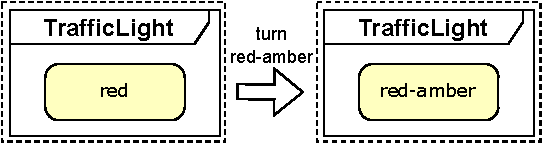
\includegraphics[width=0.35\textwidth]{figures/sm_rule.pdf}
    \caption{\gls*{gt} rules for \textit{turn green} and \textit{turn red}}
    \label{fig:sm_rule}
\end{figure}

Using a traffic light snapshot with the state red as a start graph, we generate the same state space in Groove as the traffic light state machine describes.
All generated \gls*{gt} systems, including further instructions regarding execution and consistency checking, can be found in \cite{krauterArtifactsBehavioralConsistency2023}.


\subsubsection{BPMN semantics}
The local \gls*{hot} to generate \gls*{gt} rules for \gls*{bpmn} processes is challenging, and we are currently only supporting a subset of the \gls*{bpmn} semantics.
Generally, we construct one or more rules for each flow node, i.e., type of state-changing element in a \gls*{bpmn} model.
Furthermore, we created a comprehensive test suite to ensure the correctness of our \gls*{hot} \cite{krauterArtifactsBehavioralConsistency2023}.
\autoref{fig:bpmn_example_rules} shows the \gls*{gt} rules for the task \textsf{Switch to P1} of the TJunction controller.
It uses the concrete syntax introduced in \cref{fig:snapshot_metamodels} to represent process snapshots containing tokens.


\begin{figure}[h]
    \centering
    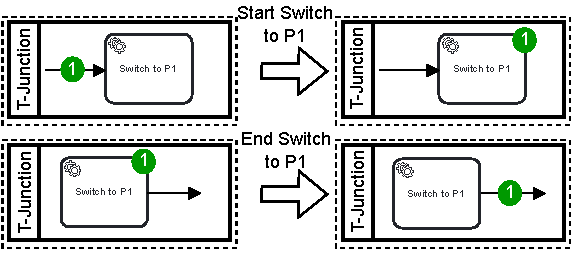
\includegraphics[width=0.475\textwidth]{figures/bpmn_rules.pdf}
    \caption{Example \gls*{gt} rules for the TJunction controller}
    \label{fig:bpmn_example_rules}
\end{figure}

Due to limited space, we only show the \textsf{Switch to P1} rules but the artifacts of this paper \cite{krauterArtifactsBehavioralConsistency2023} contain the full \gls*{gt} system and a wiki explaining the \gls*{hot} in detail.
To summarize, we can generate \gls*{gt} systems that implement the behavioral semantics of \gls*{bpmn}.


\subsubsection{Check behavioral consistency}
The defined interactions change the rules for switching to phases 1 and 2.
\autoref{fig:global_rule} shows the resulting rule for switching to phase 1.
We decided that the interactions between the traffic lights and the TJunction controller should synchronize with the end of the task, not the start.
Thus, the rule was constructed using the individual rules \textit{turn green} and \textit{turn red} for traffic lights (see \cref{fig:sm_rule}) and the rule \textit{End Switch to P1} (see \cref{fig:bpmn_example_rules}).
Exactly these rules were used since they are generated from the state-changing elements specified in the first interaction (see \cref{lst:interactions}).

\begin{figure}[h]
    \centering
    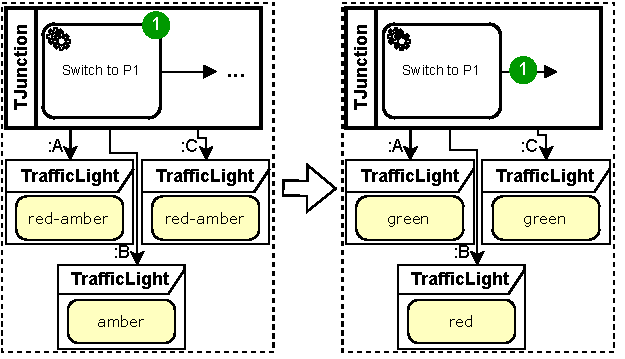
\includegraphics[width=0.475\textwidth]{figures/global_rule.pdf}
    \caption{Global \gls*{gt} rule to switch to phase 1}
    \label{fig:global_rule}
\end{figure}

The rule changes all traffic lights simultaneously and finishes the task.
The corresponding individual rules no longer exist, so synchronization of the behavior is guaranteed.
A similar rule exists for switching to phase 2, resulting from the other interaction.
All other rules are left untouched while constructing the global \gls*{gt} system.

Finally, we can generate the global state space of the system using the global \gls*{gt} system, which can be found in \cite{krauterArtifactsBehavioralConsistency2023}.
To check the requirements formalized by properties 1-4, we must also encode the used atomic propositions.
These are specified as \textit{graph conditions} in Groove.
A graph condition in Groove is a rule that does not change elements but can be used as an atomic proposition in model checking.

\subsection{Behavioral consistency in the use case}
Running the obtained \gls*{gt} specification shows that properties \eqref{eq:property1} and \eqref{eq:property2} hold, while properties \eqref{eq:property3} and \eqref{eq:property4} do \textit{not} hold (see artifacts in \cite{krauterArtifactsBehavioralConsistency2023}).
The counterexamples for properties 3 and 4 show an unexpected race condition that must be handled:
After the TJunction controller signals that the traffic light A/B is green, bus B1/B2 can advance to the \textsf{Pass Junction} activity.
However, simultaneously, the TJunction controller can enter the subprocess for the next phase, which can be interrupted by the associated timer event.
This can happen before bus B1/B2 passes the junction, resulting in an invalid state.

The system developers have different options to handle the detected inconsistencies.
One option is to keep the models unchanged and pay special attention to the found race condition during system implementation.
This can be an acceptable solution since the \textsf{Pass Junction} activity is also modeled as a user activity, i.e., the bus driver decides when to cross the T-Junction.
Furthermore, tolerating inconsistencies can be a viable option in \gls*{mde} \cite{weidmannToleranceModelDrivenEngineering2021}.
Another option is to change the models to resolve the inconsistency.
For example, the T-Junction controller could wait for the bus to pass before changing the traffic lights again.

\section{Discussion} \label{sec:discussion}
In this section, we discuss two potential limitations of our approach: supporting new modeling languages and state space explosion.

\subsection{Support for new modeling languages}
To support a new modeling language in our approach one has to do the following: describe the state structure in a snapshot metamodel, identify state-changing elements in the language's metamodel, and implement a \gls*{hot} to the chosen formalism.
A plugin containing these three artifacts can then be reused.

Implementing a \gls*{hot} that correctly implements a new modeling language's semantics takes time and effort.
We learned that when implementing \glspl*{hot} to the same underlying formalism, one gets accustomed to the formalism and naturally builds a framework to generate and test specifications in this formalism.
Thus, the work needed to implement new languages decreases over time, but one must always understand the semantics of a new language to map them to the chosen formalism.


\subsection{State space explosion}
State space explosion is one of the predominant issues when applying model checking to complex systems, which are often found in real-world applications.
As one can see in \cref{table:grooveRuntime} and \cref{table:maudeRuntime}, our approach is not immune to state space explosion.
The tables show the states, transitions (rewrites), and average runtime of a full state space exploration in the Groove (Maude) specification.
Four scenarios were benchmarked, starting with the use case multi-model without approaching buses and then increasing the number of buses up to three.

To calculate the average runtime, we used the hyperfine benchmarking tool \cite{peterHyperfine2022} (version 1.15.0), which ran state space exploration for each scenario ten times.
Timing evaluations were done with an AMD Ryzen 7700X processor and 32 GB of RAM running Maude version 3.1 (inside the Windows Subsystem for Linux) and Groove version 5.8.1.
A description of how to run the benchmarks is available in \cite{krauterArtifactsBehavioralConsistency2023}.

Generally, the Maude exploration time is lower despite larger state spaces due to technical differences in implementing the \gls*{bpmn} semantics.
However, as expected, neither of the tools is immune to state space explosion.

\begin{table}[ht]
\centering

\begin{tabular}{|c || c | c | c |}
 \hline
 Use case & States & Transitions & Exploration time \\
 \hline\hline
 No buses & 168 & 438 & \textasciitilde 1.201 ms \\
 \hline
 1 bus & 2.888 & 10.046 & \textasciitilde 1.647 ms \\
 \hline
 2 buses & 27.880 & 121.554 & \textasciitilde 4.087 ms \\
 \hline
 3 buses & 195.336 & 1.028.340 & \textasciitilde 25.137 ms \\
 \hline
\end{tabular}
\caption[State space exploration in Groove]{State space exploration in Groove}
\label{table:grooveRuntime}

\smallskip

\begin{tabular}{|c || c | c | c |}
 \hline
 Use case & States & Rewrites & Exploration time \\
 \hline\hline
 No buses & 168 & 664 & \textasciitilde 28 ms \\
 \hline
 1 bus & 3.304 & 19.958 & \textasciitilde 120 ms \\
 \hline
 2 buses & 35.280 & 279.776 & \textasciitilde 1.279 ms \\
 \hline
 3 buses & 260.176 & 2.522.582 & \textasciitilde 12.599 ms \\
 \hline
\end{tabular}
\caption[State space exploration in Maude]{State space exploration in Maude}
\label{table:maudeRuntime}

\end{table}

% Discussion
% Full state space is not what you do. You check properties.
As in our use case, one is generally not interested in a full state space exploration as in \cref{table:grooveRuntime} and \cref{table:maudeRuntime} but rather in the validity of a set of behavioral properties.
Checking a property specified in \gls*{ltl} does not necessarily lead to a full state space exploration.
Furthermore, not every property is concerned with all behavioral models.
For example, properties (1) and (2) of the use case do not involve buses and can be checked on smaller state spaces, not including approaching buses.
In addition, checking a set of properties can be run in parallel.
If some properties are computationally expensive, they can be run on dedicated hardware, for example, during a continuous integration pipeline once a day in case of a behavioral model or interaction change.
Thus, checking the consistency of a multi-model can be seen as an additional test during \gls*{mde}, which can be run locally but, in addition, is a vital part of continuous integration.

% Ways to mitigate state space explosion.
The performance of the Maude \gls*{ltl} model checker is comparable to the popular SPIN model checker \cite{ekerMaudeLTLModel2004} and thus is proven to be competitive.
However, one could use different techniques to mitigate the state space explosion problem further.
One technique is to abstract models further such that they only contain information relevant to the set of properties to be checked.
Thus, minimal models are synchronized, leading to smaller state spaces.
However, finding correct minimal models might not be trivial.

Partial-order reduction is a well-known and effective technique to mitigate the state space explosion problem.
It is currently not implemented in the Maude LTL model-checker, but there is promising work to integrate partial-order reduction into the model-checker \cite{farzanPartialOrderReduction2007}, showing substantial state space reductions.
The potential to reduce the state space using this technique is huge, especially for model-checking concurrent systems \cite{clarkeHandbookModelChecking2018}.
Our approach analyzes concurrent systems with some interaction, and thus model-checking would greatly benefit from partial-order reduction.
In our opinion, partial-order reduction must be implemented to analyze models from real-world applications.


\section{Related work} \label{sec:related_work}
This contribution builds on our previous publication \cite{krauterBehavioralConsistencyHeterogeneous2021}.
However, we refined the behavioral consistency management workflow into five steps and introduced new key concepts such as state, state-changing elements, interactions, and behavioral relationships.

% Intro to the following sections
We organized related work into two sections.
First, we discuss ad-hoc and general solutions related to the problem of behavioral consistency.
Then, we relate our work to the fields of \gls*{mpm} and co-simulation.

\subsection{Ad-hoc and general solutions}
% Highlight some specific combinations/ad-hoc approaches for a single modeling language.
The general idea of transforming different behavioral formalisms to a single formalism to reason about cross-cutting concerns is not new, see, e.g., \cite{engelsMethodologySpecifyingAnalyzing2001}.
For example, \cite{kusterExplicitBehavioralConsistency2003} developed consistency checking for sequence diagrams and statecharts based on \gls*{csp}, while \cite{yaoConsistencyCheckingUML2006} used Petri nets for the same scenario.
Nevertheless, these approaches only resemble ad-hoc solutions to specific combinations of two languages.
They do not consider the general problem of behavioral consistency in a heterogeneous modeling scenario.

% Kienzle with event structures: composition
\cite{kienzleUnifyingFrameworkHomogeneous2019} proposes a unifying framework for homogeneous model composition of structural and behavioral models.
To combine behavioral models, they use Event structures as an underlying formalism and show how different homogeneous behavioral models can be combined.
In addition, to express behavioral relationships between different models they create causal relationships, which are used during model composition. 
In the future, they plan to apply their framework to combine heterogeneous models but have not done so yet. 
Generally, their approach is compatible with ours since we do not mandate a specific formalism.
Thus, Event structures could be considered, where interactions are realized using causal relationships.
Since their research challenges and resulting work items align with our work, we see our work following the same line of research.
In addition, they cover the same class of behavioral formalisms as our approach (see \acrshort*{devs} in the next subsection).

\cite{varalarsenBehavioralCoordinationOperator2015} propose the coordination language B-COoL.
In B-COoL a user defines behavioral interfaces for each behavioral language, which are then used to specify interactions between models.
To execute the models with the specified interactions, they transform them into \gls*{ccsl} models.  
Their work results in plugins for GEMOC studio, which support running and debugging the models.

Both approaches are similar to our approach since both have mechanisms to define interactions between behavioral models and generate a global behavioral specification based on these interactions.
Furthermore, the generation of the global behavior is achieved by transforming models to a certain formalism like the \gls*{hot} in our approach.
However, the generated specification does not allow to check global behavioral properties since they do not make the state structure (snapshot metamodels in our approach) of the participating models explicit.
In this paper, we identified the two fundamental concepts: \textit{state} and \textit{state-changing elements} to check behavioral consistency when heterogeneous models interact.

\subsection{Multi-paradigm modeling and co-simulation}
% Introduce MPM. 
\gls*{mpm} is based on the idea to model every aspect and part of a system using the most appropriate modeling formalism(s) \cite{amraniMultiparadigmModellingCyber2021}.
Thus, \gls*{mpm} often leads to multi-modeling scenarios where models conforming to different modeling formalisms are used.

Different behavioral formalisms can be classified using two criteria: \textit{time} and \textit{values of state variables} \cite{wainerDiscreteeventModelingSimulation2009}.
\Cref{fig:classification} shows the classification where time and state variables can either be \textit{discrete} or \textit{continuous}.
% Co-Simulation is a subfield of this, i.e., running the models modeled in multiple paradigms together.

\begin{figure}[ht!]
    \centering
    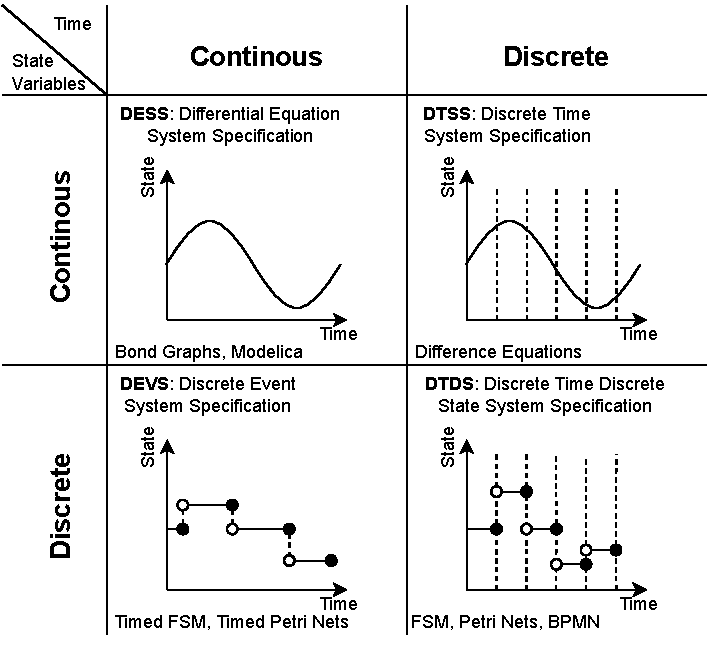
\includegraphics[width=0.49\textwidth]{figures/diagrams-classification.pdf}
    \caption{Classification of behavioral formalisms according to the nature of the \textit{time} and \textit{state variables} (adopted from \cite{wainerDiscreteeventModelingSimulation2009, amraniMultiparadigmModellingCyber2021})}
    \label{fig:classification}
\end{figure}

% We only support formalisms where states are discrete (lower part).
So far we have seen \glspl*{dtds} like \gls*{fsm} and \gls*{bpmn} in this work, where time and state variables are discrete.
Furthermore, our approach can be applied to \glspl*{devs} since the underlying formalisms support continuous time, see for example \cite{olveczkyRealTimeMaudeIts2014}.
However, we do not support formalisms with continuous state variables (top part of \cref{fig:classification}), since our central concept of \textit{state-changing elements} would need to be changed.
We think that supporting \gls*{devs} formalisms is a good trade-off between the usefulness and complexity of our approach, since \gls*{devs} covers a wide variety of formalisms \cite{vangheluweIntroductionMultiparadigmModelling2002}.

Due to the use of different modeling formalisms system simulation when following the \gls*{mpm} paradigm is not an easy task.
Co-Simulation aims to solve this problem by composing the simulation of a system's parts into a global simulation \cite{gomesCoSimulationSurvey2019}.

For example, \cite{ekerTamingHeterogeneityPtolemy2003} propose an actor-oriented co-simulation approach, where each system part is represented as an actor.
An actor can communicate through its interfaces with other actors.
Their approach is implemented in the tool \textit{Ptolemy} and supports continuous time and state variables.
% FMI/FMU standard
Furthermore, the \gls*{fmi}\footnote{\url{https://fmi-standard.org/}} is a co-simulation standard to exchange executable systems parts, so-called \glspl*{fmu}.
Each \gls*{fmu}, similar to the actors in Ptolemy, comes with an XML model to describe its interface, for example, the \gls*{fmu}'s exposed variables.
\glspl*{fmu} support continuous time and state variables and are widely used in the industry.

However, with co-simulations, one can only simulate systems not check global behavioral properties.
Our approach supports global properties by introducing the two fundamental concepts: \textit{state} and \textit{state-changing elements} and only allowing formalisms with discrete state variables.

\section{Conclusion and future work} \label{sec:conclusion_and_future_work}
% Conclusion
Our work represents the first formalization of behavioral consistency management in a heterogeneous modeling scenario, enabling formulating and checking \textit{global} properties.
Previous work either only dealt with the behavioral consistency between specific pairs of models or focused on the simulation in a heterogeneous scenario but lacked checking global properties.

Our approach is based on two fundamental concepts: \textit{state} and \textit{state-changing elements}.
The state structure of each participating behavioral language must be explicitly defined such that we can infer how global states are structured.
Furthermore, state-changing elements serve as a minimal behavioral interface to uniformly define interactions for heterogeneous models.
These two fundamental concepts can be found in most, if not every \gls*{devs} formalism.
Thus, our approach can support behavioral formalisms with discrete state variables.

In future work, we plan to extend our implementation to support more behavioral formalisms such as activity diagrams, hierarchical state machines, and the $\pi$-calculus.
In addition, we aim to apply the approach to real-life industrial case studies.
% Data transfer
Furthermore, two systems often exchange data while interacting, for example, using name-passing or messaging.
The exchanged data then greatly influences the future behavior of the systems.
Thus, adding data transfers to interactions between heterogeneous models is an important issue left for future work.
% Consistency restoration
Finally, if consistency violations are found, consistency restoration must be achieved.
We leave consistency restoration of behavioral models as a problem for future work.

\begin{figure}[ht!]
    \centering
    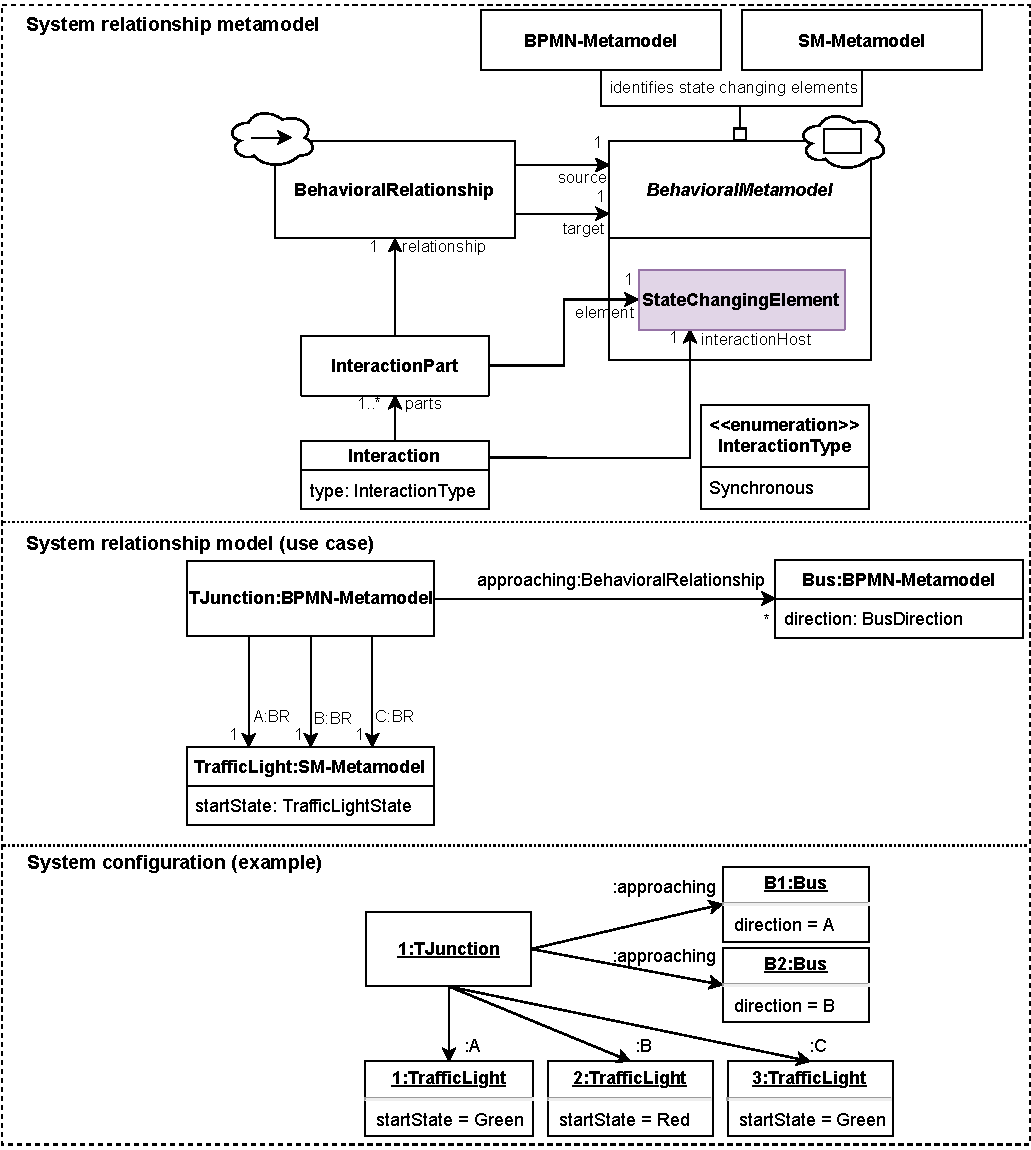
\includegraphics[width=0.5\textwidth]{figures/allConcepts.pdf}
    \caption{Overview of all concepts and their usage}
    \label{fig:allConcepts}
\end{figure}
% Change SRM Syntax to not look like a class diagram? Open question/discussion.

\bibliography{bib}

\section*{About the authors}

\shortbio{Tim Kräuter}{is a Ph.D. student at the Western Norway University of Applied Sciences, Bergen, Norway.
His primary research is on integrating heterogeneous behavioral models in multi-model-driven software engineering.
Previously he worked as a software developer and acquired a master of science in Information Engineering at the University of Applied Sciences, FHDW Hannover, Germany.
\authorcontact[https://timkraeuter.com/]{tkra@hvl.no}}

\shortbio{Harald König}{is a professor for Computer Science at the University of Applied Sciences, FHDW Hannover, Germany, and an Adjunct Professor at the Department of Computer Science, Electrical Engineering and Mathematical Sciences at the Western Norway University of Applied Sciences, Bergen, Norway.
Before entering academia, he worked at SAP in Walldorf and received his Ph.D. in pure Mathematics from Leibniz University in Hannover, Germany. \authorcontact{harald.koenig@fhdw.de}}

\shortbio{Adrian Rutle}{is a professor at the Department of Computer science, Electrical engineering and Mathematical sciences at the Western Norway University of Applied Sciences, Bergen, Norway.
Rutle’s main interest is applying theoretical results from the field of model-driven software engineering to practical domains and his main expertise is in the development of formal modeling frameworks for domain-specific modeling languages, graph-based logic for reasoning about static and dynamic properties of models, and the use of model transformations for the definition of the semantics of modeling languages.
His recent research focuses on multilevel modeling, model repair, multi-model consistency management, modeling and simulation for robotics, digital fabrication, smart systems, and applications of machine learning in model-driven software engineering.
\authorcontact{aru@hvl.no}}

\shortbio{Yngve Lamo}{is a professor at the Department of Computer science, Electrical engineering and Mathematical sciences at the Western Norway University of Applied Sciences, Bergen.
Lamo holds a Ph.D. in Computer Science from the University of Bergen, Norway. His research interests span from formal foundations of Model-Based Software Engineering to its applications, especially in Health Informatics.
He is currently applying MDSE to create Adaptive Software Technologies for mental Health. \authorcontact{yla@hvl.no}}

\shortbio{Patrick Stünkel}{is currently working as a postdoctoral researcher at Haukeland University Hospital in Bergen, Norway, where he is working on applying process mining, workflow modeling, and optimization techniques in digital pathology.
Before that, Patrick did his Ph.D. at Western Norway University of Applied Sciences on the topics of semantic interoperability and consistency management among heterogeneous software models.
\authorcontact[https://past.corrlang.io/]{Patrick.Stunkel@helse-bergen.no}}

\end{document}